\section{IO Tests}
Before our \gls{pcb} board arrived we tested each subsystem separately.
During testing the group gained valuable experience about all the subcomponents and how they interacted with each others.

\subsection{DAC}

\subsubsection{Without the PCB}

The \gls{dac} was tested prior to \gls{pcb} arrival, to ensure correct operation from an \gls{fpga}.
Eight wires were soldered onto the \gls{dac}, and connected to a breadboard.
The \gls{fpga} was flashed with and simple architecture, which repeatedly read the status of 14 general I/O pins, and shifted each bit out sequentially on another pin.
Both the \gls{dac} and \gls{fpga} clock input was driven by an external frequency generator, producing 3.3VPP at 10MHz.

To validate the signal output from the \gls{fpga} a logical analyser was used.

With VRef and /(V_{DD}/) at 5.0V, the analogue \gls{dac} output was measured to 0.69V when no data signal was asserted, and 2.8V when the \gls{msb} was asserted. This small offset, is the result of some of the lower order bits being left unconnected.

\subsubsection{With the PCB}

Once the the \gls{pcb} arrived we were able to test the \gls{dac}s soldered onto the \gls{pcb} as well as with actual data from the \gls{fpga}.

Clocking data from the \gls{fpga} to the \gls{dac}s on our \gls{pcb} presented some issues as we hit a limit in the Spartan-6 architecture regarding clock routing. This was resolved by using an ODDR\cite[pp. 61--65]{fpga-io} in order to forward the clock signal to the desired output pin.


\subsection{Oscilloscope}
As a proof of concept to draw on an oscilloscope, we created a 4-bit resistor ladder \gls{dac}. The schematic of the \gls{dac} is displayed in Figure \ref{fig:r2r-ladder}.
An Arduino was used to control the \gls{dac}.

To test drawing on both x-axis and y-axis, the circuit consisted of 2 4-bit \gls{dac}s.
With a small Arduino program we were able to draw a square, depicted in Figure \ref{fig:osc_poc}.
When the Arduino changed the voltage on its \gls{gpio} pins, there was a voltage drop across all pins.
The consequence of the voltage drop is clearly visible (see Figure \ref{fig:osc_poc}).


\begin{figure}[h]
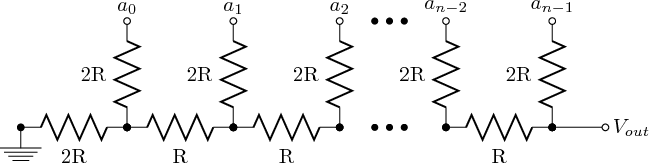
\includegraphics[width=\columnwidth]{images/r2r-ladder}
\centering
\caption{Schematics of the resistor-ladder\cite{r2r-ladder-schematics}.}
\label{fig:r2r-ladder}
\end{figure}

\begin{figure}[h]
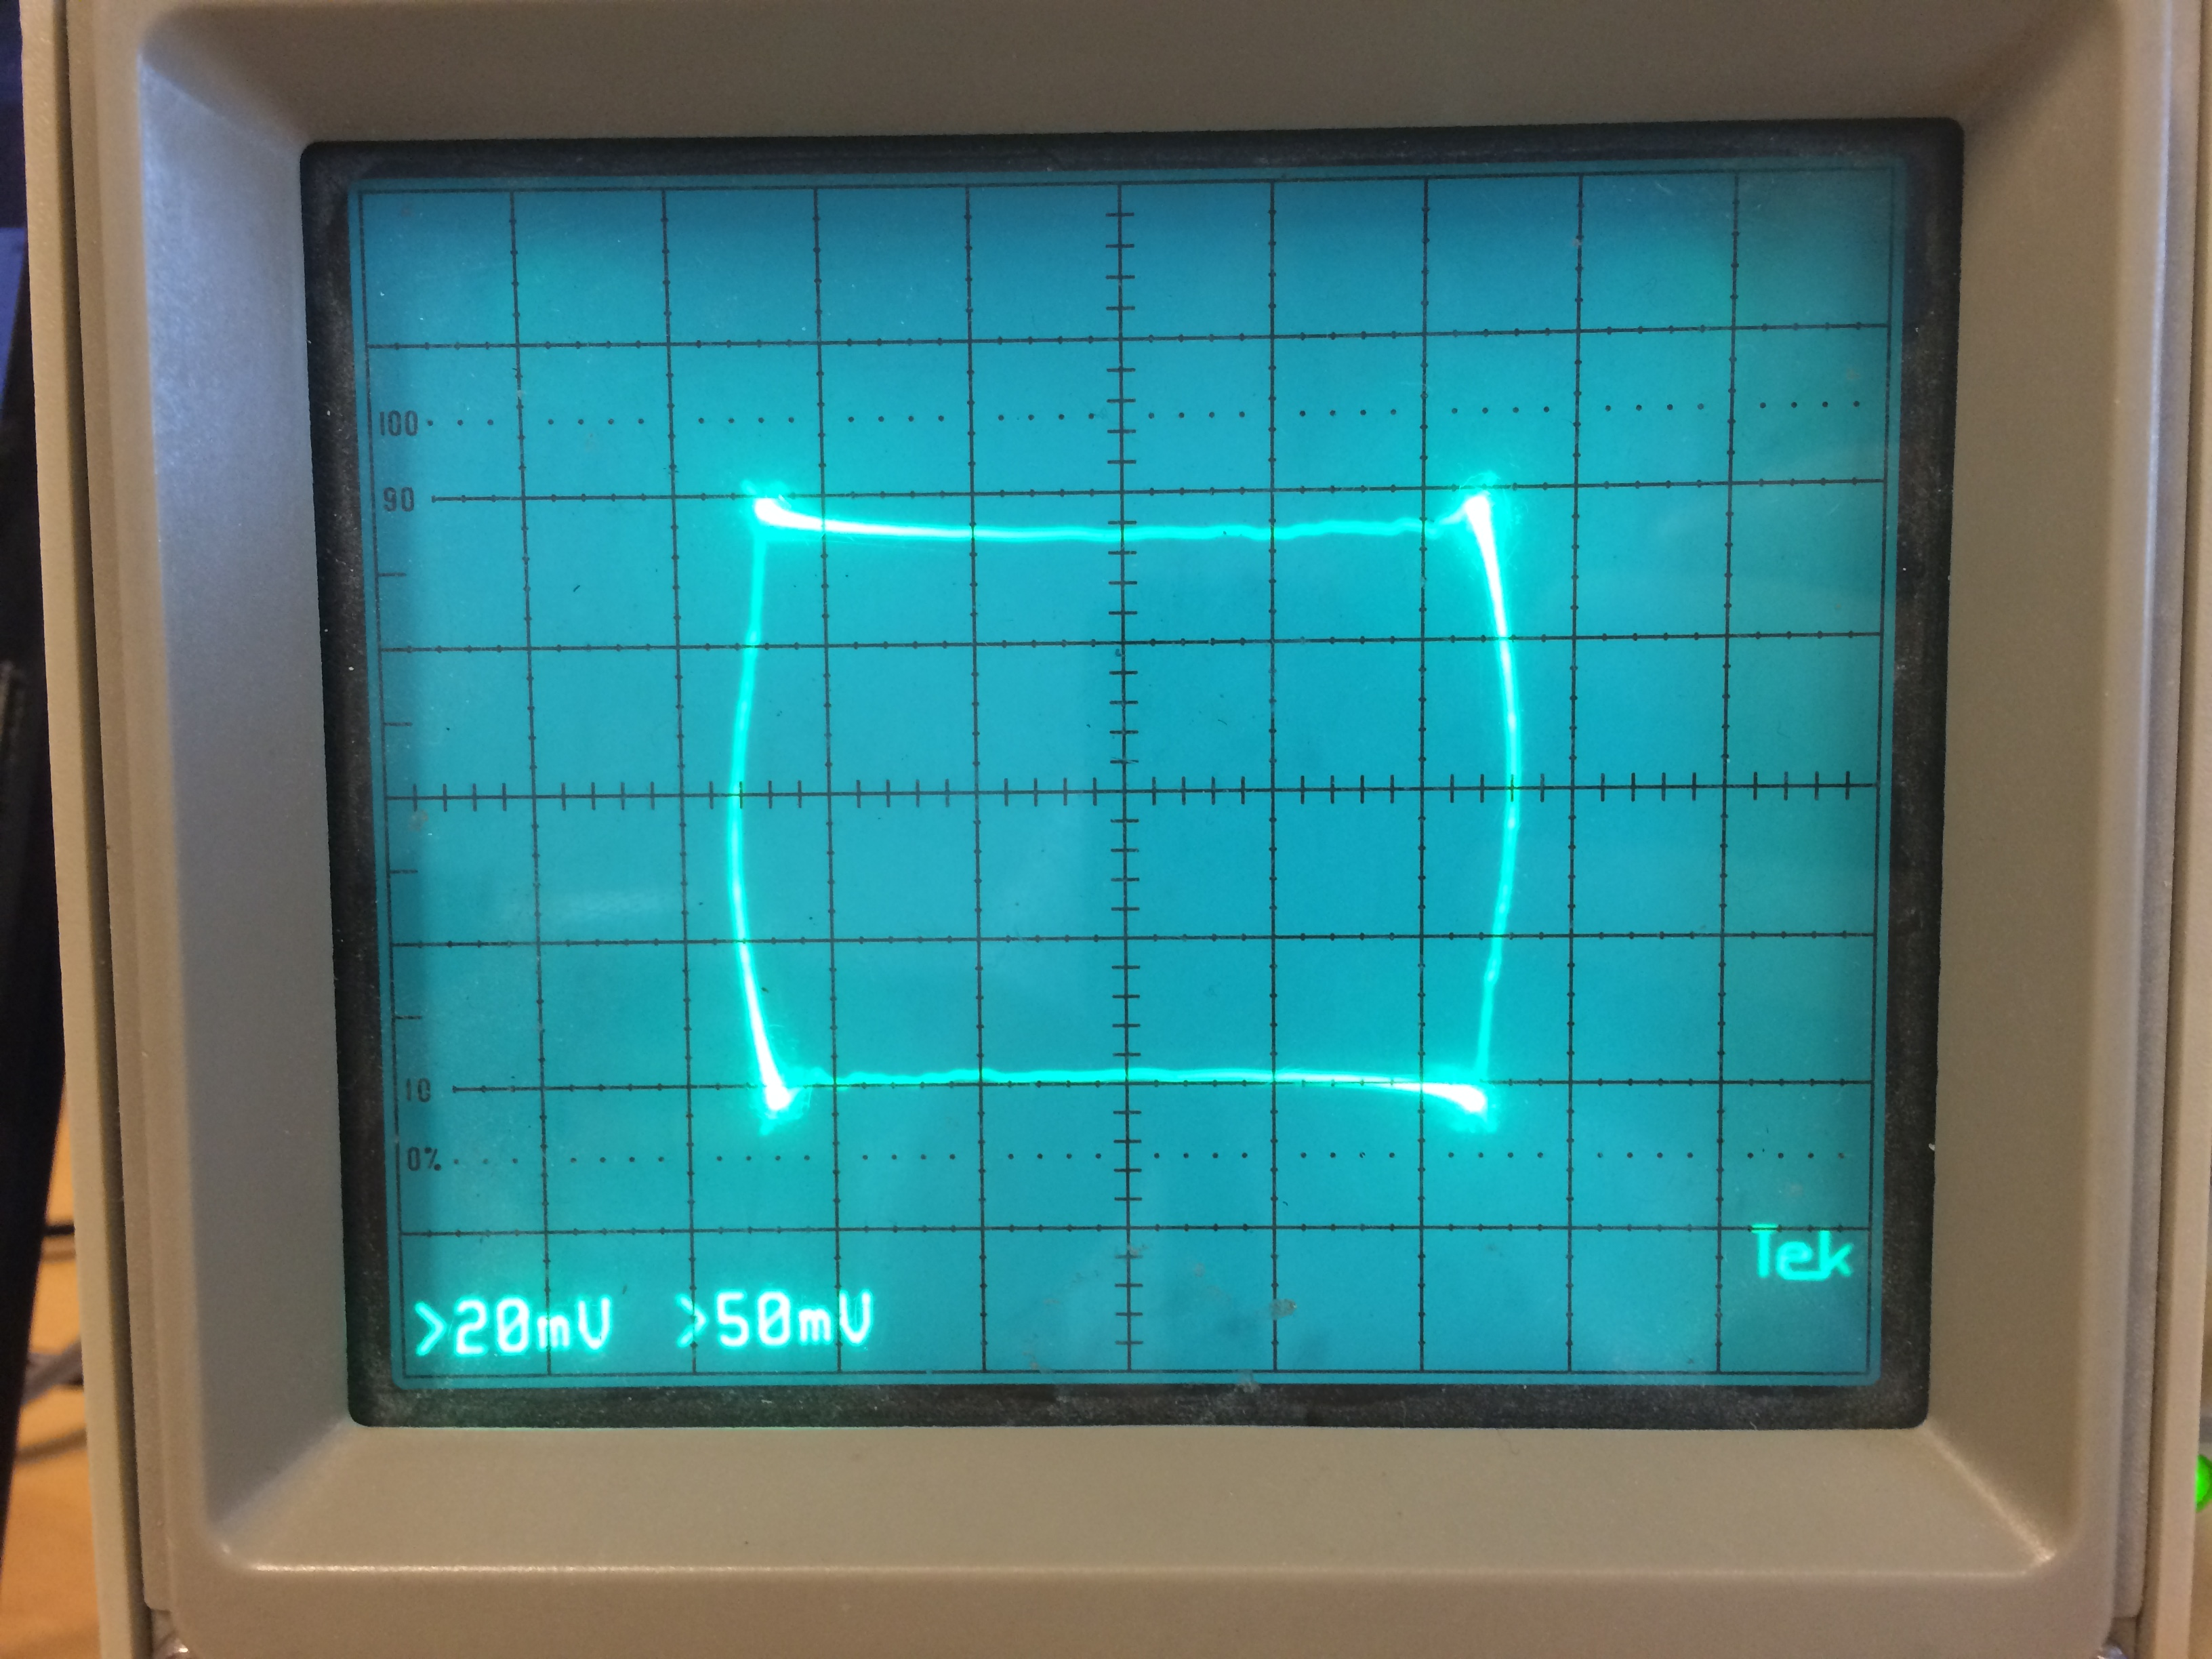
\includegraphics[width=\columnwidth]{images/osc_square_close}
\centering
\caption{A "square" drawn on the oscilloscope using an Arduino and two resistor-ladder \gls{dac}s}
\label{fig:osc_poc}
\end{figure}